\documentclass[10pt,nocombine]{leaflet}







\usepackage[T1]{fontenc}
\usepackage{libertine}
\renewcommand{\familydefault}{\sfdefault}
\usepackage{microtype}
\usepackage{graphicx}
\graphicspath{{}}
\pagenumbering{gobble}
\usepackage{xcolor}
\renewcommand{\sectfont}{\Large\sffamily\bfseries\color{cobalt}}
\usepackage{enumitem}
\usepackage{setspace}
\usepackage{fontawesome}
\usepackage{amssymb}
\usepackage{transparent}



\usepackage{pgf}
\usepackage{pgfkeys}
\usepackage{circledsteps}
\usepackage{tikz}
\usetikzlibrary{arrows.meta}
\usetikzlibrary{decorations.markings}
\AddToBackground{5}{%
\put (0,0) {\transparent{1}\hspace{-9.9cm}\scalebox{-1}[1]{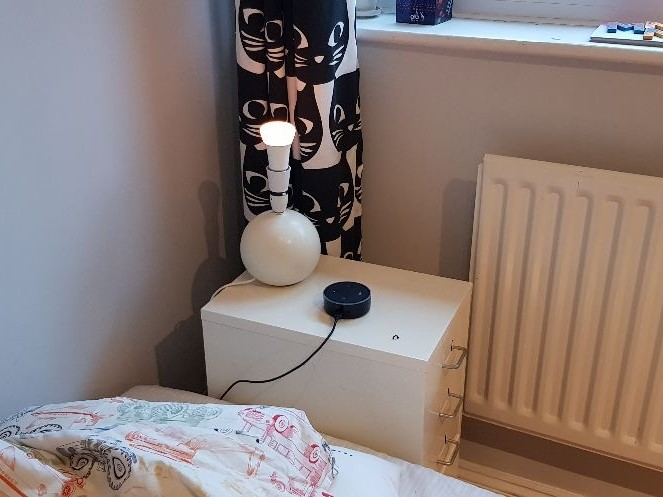
\includegraphics[width=29.7cm]{figures/h4-2.jpg}}}
{\transparent{.5}\tikz\fill[color=illuminating] (0,0) rectangle (9.9cm,6cm);}
}

\AddToBackground{6}{%
\put (0,0) {\transparent{0.5}\hspace{-19.8cm}\scalebox{-1}[1]{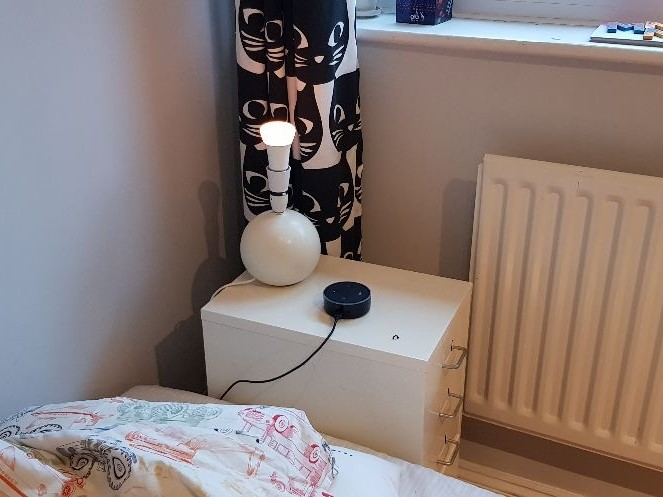
\includegraphics[width=29.7cm]{figures/h4-2.jpg}}}
\tikz\fill[fill=illuminating,fill opacity=.5] (0,0)  rectangle (9.9cm,\paperheight);
}

\AddToBackground{4}{%
{\transparent{0.3}
\includegraphics[height=21cm]{figures/wood background.png}}
}

\definecolor{illuminating}{HTML}{F5DE4C}
\definecolor{cobalt}{HTML}{2613A8}
\definecolor{mdpurple}{HTML}{7B5E80}
\definecolor{cyanblue}{HTML}{624CF5}


\AddToBackground{1}{%

\begin{tikzpicture}
{\transparent{1}\fill[fill=illuminating] (0,0)  rectangle (9.9cm,\paperheight);}
\end{tikzpicture}
}
% \AddToBackground{5}{%
% \begin{tikzpicture}
% \fill[fill=purple,fill opacity=.7] (0,0)  rectangle (9.9cm,\paperheight);
% \end{tikzpicture}
% }


\begin{document}
\pagestyle{plain}
\pagenumbering{arabic}
\thispagestyle{empty}

\begin{center}
    \onehalfspacing
   \color{black} \huge\textbf{Responsible \\ Digital Housekeeping}
\end{center}


\vfill
\begin{center}
\color{black}\fontsize{80}{80}\faGroup    
\end{center}




\begin{center}
\singlespacing
\fontsize{40}{40}\selectfont \color{black}\bfseries How to be `at home' with smart devices
\end{center}

\vfill

\begin{center}
\onehalfspacing
\huge \bfseries \itshape A Guide\\[2ex]
\fontsize{40}{40}\faHandORight
\end{center}

\clearpage
\section{10 Facts on People and Technology}
\vfill
\begin{onehalfspacing}
\pgfkeys{/csteps/fill color=illuminating}
\pgfkeys{/csteps/outer color=illuminating}
\pgfkeys{/csteps/inner color=black}
\pgfkeys{/csteps/inner ysep=10pt}
\pgfkeys{/csteps/inner xsep=10pt}
\begin{enumerate}[label=\Large\protect\Circled{\bfseries\normalsize\arabic*},labelsep=10pt,leftmargin=40pt]
    \item \large How interesting or appealing a device appears is entirely subjective.\vspace{1ex}
    \item \large It is common to share personal devices and use shared devices at home.\vspace{1ex}
    \item \large Our past experience influences how well we `get on' with new devices.\vspace{1ex}
    \item \large Solving others' problems \textit{without} their involvement induces dependence.\vspace{1ex}
    \item \large Technology design entices playful behaviour to discover features and services.\vspace{1ex}
    \item \large Using smart technology responsibly is difficult for adults and children.\vspace{1ex}
    \item \large Despite best efforts, unanticipated problems occur and need to be dealt with.\vspace{1ex}
    \item \large Smart technology requires regular housekeeping. Housekeeping takes time.\vspace{1ex}
    \item \large People find their own creative ways of using smart devices.\vspace{1ex}
    \item \large Not interacting with technology does not mean not caring about what it does.
\end{enumerate}
\end{onehalfspacing}
\vfill

\clearpage

\section{\color{cobalt}Make Things Run Smoothly}
\vfill
\begin{onehalfspacing}\large
Good news! -- There is a lot you can do during setup, configuration, and use to make tech work for everyone!
\end{onehalfspacing}
\vfill
\rotatebox[]{0}{
\parbox{\linewidth}{
\centering
\tikzset{
    myarrow/.style={
        decoration={markings,mark=at position 0.999 with {\arrow[scale=2]{>}}},
        postaction={decorate},
        >=stealth
    },
    myarrowstraight/.style={
        decoration={markings,mark=at position 1 with {\arrow[scale=2]{>}}},
        postaction={decorate},
        >=stealth
    },
}
\begin{tikzpicture}[scale=.9]
\pgfkeys{/csteps/fill color=illuminating}
\pgfkeys{/csteps/outer color=illuminating}
\pgfkeys{/csteps/inner color=black}
\pgfkeys{/csteps/inner ysep=10pt}
\pgfkeys{/csteps/inner xsep=10pt}
\draw[decoration={markings,mark=at position 0.65 with {\arrow[scale=2]{>}}},
        postaction={decorate}] (9,1.7) circle (1.7cm);
\draw[decoration={markings,mark=at position 0.65 with {\arrow[scale=2]{>}}},
        postaction={decorate}] (6,1.7) circle (1.7cm);

%  \node[] (discovery) at (0,0) {discovery};
 
 \node[] (purchases) at (3.5,0) {\itshape... purchase};
 
 \node[rectangle,fill=white] (setup) at (6,0) {\itshape\shortstack{setup \&\\ configu-\\ration}};
 
 \node[rectangle,fill=none] (expectations) at (6,3) {\bfseries\shortstack{\large\Circled{\faBullseye~A}\\expectations}};
 
 \node[rectangle,fill=white] (purpose) at (7.5,1.7) {\bfseries\shortstack{\large\Circled{\faBullseye~B}\\purpose}};
 
 \node[rectangle,fill=none] (empower) at (9,3) {\bfseries\shortstack{\large\Circled{\faBullseye~C}\\empowerment}};
 
 \node[rectangle,fill=white] (use) at (9,0) {\itshape use};
 
 \node[] (removal) at (10.5,0) {...};
 
 \path[draw=black,decoration={markings,mark=at position 1 with {\arrow[scale=2]{>}}},
        postaction={decorate}] (purchases) -- (setup) -- (use) -- (removal) -- (11.5,0);



\end{tikzpicture}

}}



\vfill
\begin{onehalfspacing}
\pgfkeys{/csteps/fill color=illuminating}
\pgfkeys{/csteps/outer color=illuminating}
\pgfkeys{/csteps/inner color=black}
\pgfkeys{/csteps/inner ysep=10pt}
\pgfkeys{/csteps/inner xsep=10pt}

\section{\itshape\color{cobalt}Your Personal Goals}
\begin{enumerate}[label=\Large\protect\Circled{\bfseries\normalsize\faBullseye~\Alph*},labelsep=10pt,leftmargin=40pt]
    \item \large Understanding \textbf{Expectations} of those living with you is essential in making a device work for the community.\vspace{1ex}\newline {\bfseries \color{cobalt} {\Large$\rightarrow$}~Talk to them!}\vspace{1ex}
    \item \large Establishing \textbf{Purpose} for the use of a specific device is key to meet expectations. \vspace{1ex}\newline {\bfseries \color{cobalt} {\Large$\rightarrow$}~Unsure? Discuss.}\vspace{1ex}
    \item \large Community member \textbf{Empowerment} is key. Help others to understand how \textit{devices mediate their relationships} online and offline. Be \textit{responsible and responsive}. \vspace{1ex}\newline {\bfseries \color{cobalt} {\Large$\rightarrow$}~How? Be approachable.}\vspace{1ex}
\end{enumerate}
\end{onehalfspacing}
\vfill

\clearpage
\section{\color{cobalt} Take Action! \textit{With your household ...}}
\phantom{a}\vfill
\begin{onehalfspacing}
\pgfkeys{/csteps/fill color=illuminating}
\pgfkeys{/csteps/outer color=illuminating}
\pgfkeys{/csteps/inner color=black}
\pgfkeys{/csteps/inner ysep=10pt}
\pgfkeys{/csteps/inner xsep=10pt}
\begin{itemize}[label=\Large\protect\Circled{\bfseries\normalsize\faUserPlus~A},labelsep=10pt,leftmargin=40pt]
    \item \large Understand what the product does.
    % \item \large Discuss how the product might be beneficial for your household.\vspace{1ex}
    % \item \large Envision how the product could be used.\vspace{1ex}
\end{itemize}
\begin{itemize}[label=~,labelsep=10pt,leftmargin=40pt]
    % \item \large Understand what the product does.\vspace{1ex}
    \item \large Discuss how the product might be beneficial for your household.
    \item \large Envision how the product could be used.\vspace{1ex}
\end{itemize}
\begin{itemize}[label=\Large\protect\Circled{\bfseries\normalsize\faUserPlus~B},labelsep=10pt,leftmargin=40pt]
    \item \large Establish an agreement over a purpose of use (e.g. to monitor a cat). 
    % \item \large Identify whether and how individual goals align with the purpose. \vspace{1ex}
    % \item \large Discuss what constitutes purposeful use of the specific device.\vspace{1ex}
    % \item \large Understand that deviating from this purpose requires a new agreement.\vspace{1ex}
\end{itemize}
\begin{itemize}[label=~,labelsep=10pt,leftmargin=40pt]
    % \item \large Establish an agreement over a purpose of use (e.g. to monitor a cat). \vspace{1ex}
    \item \large Identify whether and how individual goals align with the purpose. 
    \item \large Discuss what constitutes purposeful use of the specific device.
    \item \large Understand that deviating from this purpose requires a new agreement.\vspace{1ex}
\end{itemize}
\begin{itemize}[label=\Large\protect\Circled{\bfseries\normalsize\faUserPlus~C},labelsep=10pt,leftmargin=40pt]
    \item \large Identify and discuss data controls (e.g. location sharing) and visualisations (e.g. logs). 
    % \item \large Approach relationships that are affected by a device: (a) discuss what data is collected and why; or (b) do not collect the data.\vspace{1ex}
    % \item \large Recognise your responsibility as digital house keeper. Be responsible and responsive.\vspace{1ex}
\end{itemize}
\begin{itemize}[label=~,labelsep=10pt,leftmargin=40pt]
    % \item \large Identify and discuss data controls (e.g. location sharing) and visualisations (e.g. logs). \vspace{1ex}
    \item \large Approach relationships that are affected by a device: (a) discuss what data is collected and why; or (b) do not collect the data.
    \item \large Recognise your responsibility as digital house keeper. Be responsible and responsive.\vspace{1ex}
\end{itemize}
\end{onehalfspacing}
\vfill
\clearpage
\phantom{a}\vfill
\parbox{\linewidth}{
{\Large\bfseries\color{cobalt} Support others by ...}
\begin{itemize}
  \large\sffamily\color{black} 
    \item showing them how you use devices.
    \item creating situations in which they can succeed.
\item encouraging and supporting their efforts.
\item creating a friendly environment.
\end{itemize}
}

% % {\Large\bfseries\color{mdpurple} In this leaflet:}
% % \begin{itemize}
% %   \large\sffamily\bfseries\color{black} 
% %     \item  Learn about people and tech.
% %     \item Establish goals to make tech work for everyone.
% % \item Understand how you can take action.

% \end{itemize}


\clearpage
{\huge\bfseries\color{cobalt} Are you ...}\\

\begin{onehalfspacing}
\flushleft
\begin{itemize}[label=\Huge\bfseries\faHome,labelsep=10pt,leftmargin=40pt]
    \item \huge using smart devices at home?\vfill
    \item \huge `taking care' of these devices?\vfill
    \item \huge the `go-to person' if something does not work?\vfill
    \item \huge facing disagreement over the use of these devices?
\end{itemize}
\end{onehalfspacing}

\vfill

\begin{onehalfspacing}
\huge\bfseries\color{cobalt} 
To make smart tech work for your home, read on.
\end{onehalfspacing}
\vspace{1cm}

\end{document}